\section{Bitmaps bewegen}\index{Bitmap!bewegen}
%\subsection{Beispiel}
In der Zusammenfassung des vorherigen Kapitels haben wir für die Darstellung von Bitmaps notiert, dass wir die linke, obere Ecke als Positionsangabe und die Höhe und Breite beispielsweise für Abstandsberechnungen brauchen. Diese Angaben lassen sich gut einem Rechteck kodieren. Pygame stellt dazu die Klasse \texttt{pygame.Rect}\myindex{pyg}{\texttt{Rect}}\randnotiz{Rect} zur Verfügung. In \abbref[vref]{picRect01} finden Sie die meiner Ansicht nach wichtigsten Attribute der Klasse.

\begin{figure}[H]
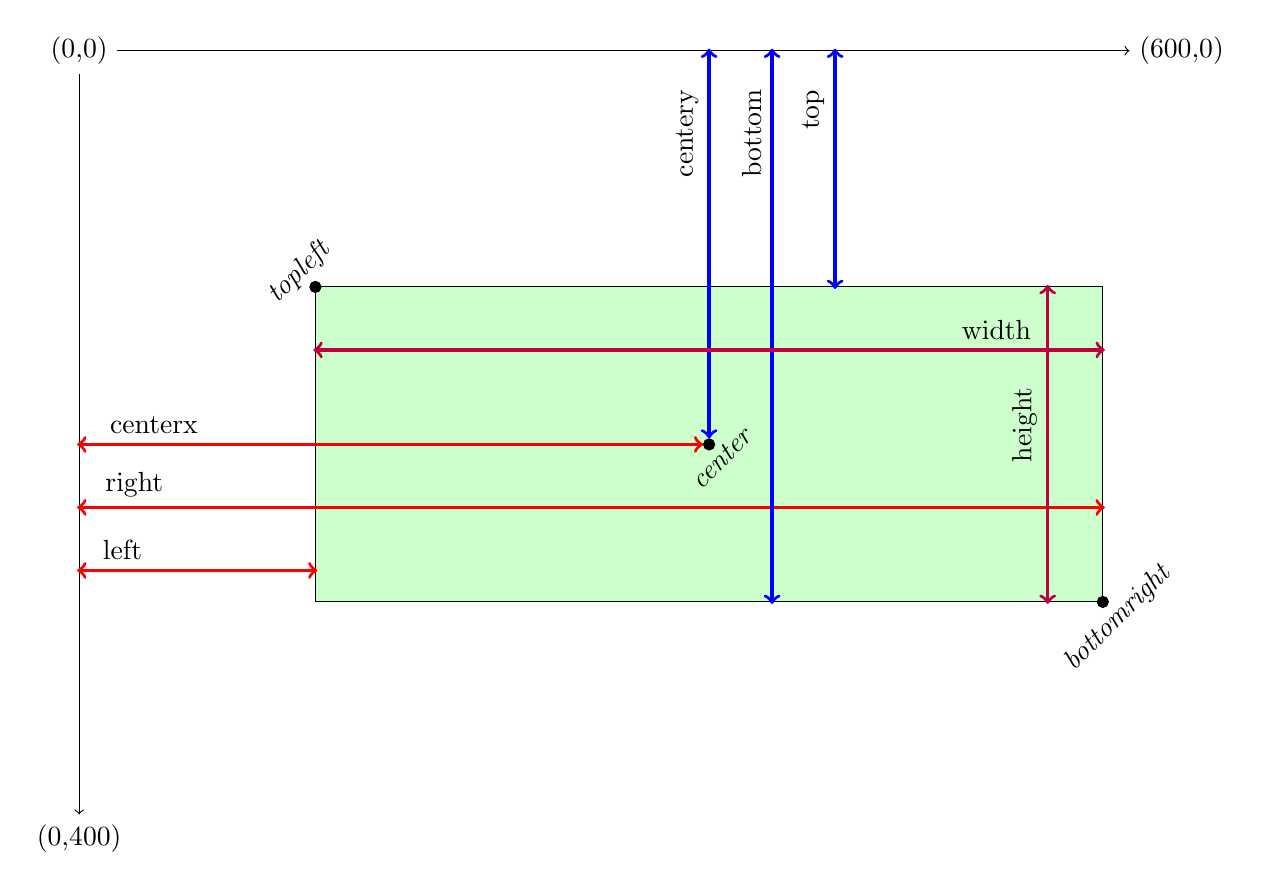
\begin{tikzpicture}
%Bildschirm Koordinatensystem
\draw
 (0,10) node (o) {(0,0)}
 (0,0) node (y) {(0,400)}
 (14,10) node (x) {(600,0)}
;
\draw[->] (o) -- (x);
\draw[->] (o) -- (y);

%Rechteck
\draw
 (3,7) node (topleft) {}
 (13,3) node (bottomright) {}
 (8.0,5) node (centerxy) {}
;
\filldraw[fill=green!20] (topleft) rectangle (bottomright);
\draw (topleft) node[above, rotate=45] {\emph{topleft}};
\draw (bottomright) node[below, rotate=45] {\emph{bottomright}};
\filldraw[fill=black] (centerxy) circle (2pt) node[below, rotate=45] {\emph{center}};
\filldraw[fill=black] (topleft) circle (2pt);
\filldraw[fill=black] (bottomright) circle (2pt);

%Left
\draw
 (-0.15,3.4) node (left1) {}
 (3.15,3.4) node (left2) {}
;
\draw[<->, very thick, red] (left1) -- (left2) node[above, black, xshift=-2.6cm] {left};


%Right
\draw
 (-0.15,4.2) node (right1) {}
 (13.15,4.2) node (right2) {}
;
\draw[<->, very thick, red] (right1) -- (right2) node[above, black, xshift=-12.45cm] {right};

%Centerx
\draw
 (-0.15,5.0) node (cx1) {}
 (8.05,5.0) node (cx2) {}
;
\draw[<->, very thick, red] (cx1) -- (cx2) node[above, black, xshift=-7.1cm] {centerx};

%top
\draw
 (9.6,10.15) node (top1) {}
 (9.6,6.85) node (top2) {}
;
\draw[<->, very thick, blue] (top1) -- (top2) node[above, black, yshift=2.4cm, rotate=90] {top};

%bottom
\draw
 (8.8,10.15) node (bottom1) {}
 (8.8,2.85) node (bottom2) {}
;
\draw[<->, very thick, blue] (bottom1) -- (bottom2) node[above, black, yshift=6.1cm, rotate=90] {bottom};

%Centery
\draw
 (8.0,10.15) node (cy1) {}
 (8.0,4.95) node (cy2) {}
;
\draw[<->, very thick, blue] (cy1) -- (cy2) node[above, black, yshift=4cm, rotate=90] {centery};

%Width
\draw
 (2.85,6.2) node (w1) {}
 (13.15,6.2) node (w2) {}
;
\draw[<->, very thick, purple] (w1) -- (w2) node[above, black, xshift=-1.5cm] {width};

%height
\draw
 (12.3,7.15) node (h1) {}
 (12.3,2.85) node (h2) {}
;
\draw[<->, very thick, purple] (h1) -- (h2) node[above, black, yshift=2.4cm, rotate=90] {height};

\end{tikzpicture}
\caption{Elemente eines \texttt{Rect}-Objekts}\label{picRect01}
\end{figure}

\myindex{pyg}{\texttt{Rect}!\texttt{centerx}}%
\myindex{pyg}{\texttt{Rect}!\texttt{right}}%
\myindex{pyg}{\texttt{Rect}!\texttt{left}}%
\myindex{pyg}{\texttt{Rect}!\texttt{centery}}%
\myindex{pyg}{\texttt{Rect}!\texttt{bottom}}%
\myindex{pyg}{\texttt{Rect}!\texttt{top}}%
\myindex{pyg}{\texttt{Rect}!\texttt{topleft}}%
\myindex{pyg}{\texttt{Rect}!\texttt{bottomright}}%
\myindex{pyg}{\texttt{Rect}!\texttt{center}}%
\myindex{pyg}{\texttt{Rect}!\texttt{width}}%
\myindex{pyg}{\texttt{Rect}!\texttt{height}}%
In der Abbildung werden Strecken in normaler Schrift und Punkte in \textit{kursiver Schrift} angegeben. Die Strecken sind eindimensional und die Punkte zweidimensional $(x,y)$. Die Koordinate~$x$ ist dabei der horizontale und~$y$ der vertikale Abstand zum 0-Punkt des Koordinatensystems. Die Bedeutung der einzelnen Angaben sollte selbsterklärend sein. Der schöne Vorteil ist, dass die Angaben sich gegenseitig berechnen. Setze ich beispielsweise \texttt{topleft = (10,10)} und \texttt{width, height = 30, 40}, so werden alle anderen Angaben für mich ermittelt. Ich muss also nicht mehr den rechten Rand mit \texttt{left + width} ausrechnen; ich kann vielmehr sofort \texttt{right} verwenden. Auch oft nützlich ist die Berechnung des Mittelpunktes \texttt{center} oder die entsprechenden Längen \texttt{centerx} und \texttt{centery}. Ändere ich nun das Zentrum durch \texttt{center = (100, 10)}, so verschieben sich alle anderen Angaben ebenfalls und müssen nicht von mir neu bestimmt werden -- sehr praktisch.

Schauen wir uns dazu eine reduzierte Version des letzten Quelltextes an. In \srcref[vref]{srcInvader05} wird die \texttt{Rect}-Klasse schon verwendet.

\lstsource{SRC/00 Einführung/04 Bewegung/invader05.py}{1}{999}{python}{Bitmaps bewegen, Version 1.0}{srcInvader05}

Für \texttt{Surface}-Objekte können wir sehr bequem mit \texttt{pygame.Surface.get\_rect()}\myindex{pyg}{\texttt{Surface}!\texttt{get\_rect()}}\randnotiz{get\_rect()} das \texttt{Rect}-Objekt erstellen lassen (\zeiref{srcInvader0501}). Die Positionierung kann nun leichter über die Attribute erfolgen. Das Zentrum muss beispielsweise nicht mehr in die Berechnung einfließen, ich kann vielmehr das horizontale Zentrum direkt als halbe Fensterbreite festlegen (\zeiref{srcInvader0502}). Auch muss die vertikale Koordinate nicht mehr vom oberen Rand aus betrachtet werden, sondern ich kann viel intuitiver den Abstand des unteren Randes vom Bildschirmrand angeben (\zeiref{srcInvader0503}). Und als Sahnehäubchen kann das \texttt{Rect}-Objekt auch noch als Parameter der \randnotiz{blit()}\myindex{pyg}{\texttt{Surface}!\texttt{blit()}}\texttt{blit()}-Funktion übergeben werden (\zeiref{srcInvader0504}).

\myebild{invader05.png}{0.8}{Bitmaps bewegen, Version 1.0}{picInvader05}

Das Ergebnis ist unspektakulär (siehe \abbref[vref]{picInvader05}) und hat noch nichts mit Bewegung zu tun.

Bewegung wird in Spielen durch veränderte Positionen animiert. Soll das Raumschiff sich nach rechts bewegen, muss sich daher die horizontale Koordinate des Schiffs erhöhen. Welche horizontale Koordinate Sie dazu verwenden -- \texttt{left}, \texttt{right} oder \texttt{centerx} --, können Sie von ihrer Spiellogik abhängig machen. In unserem Beispiel ist das egal; ich nehme daher \texttt{left}.

\lstset{firstnumber=36}
\begin{lstlisting}
defender_rect.left = defender_rect.left + 1
\end{lstlisting}

Allein diese kleine Ergänzung lässt unser Raumschiff nun nach rechts wandern. Die \texttt{+1} kodiert dabei zwei Informationen: 
\begin{itemize}
	\item \textbf{Richtung:}\randnotiz{Richtung}\index{Richtung} Hier ist das Vorzeichen \texttt{+}. Dadurch erhöht sich die Angabe \texttt{left} bei jedem Schleifendurchlauf; der linke Rand -- und damit die ganze Grafik -- der Grafik wandert damit nach rechts. Wollte man nach links wandern, müsste das Vorzeichen~\texttt{-} sein. Die horizontale Koordinate wird dadurch immer kleiner und nähert sich damit der~0. Völlig analog würde das Vorzeichen die Richtung in der Vertikalen steuern. Ein~\texttt{+} würde die Grafik nach unten und ein~\texttt{-} nach oben bewegen. Probieren Sie es aus!
	
	\item \textbf{Geschwindigkeit:}\randnotiz{Ge\-schwin\-dig\-keit}\index{Geschwindigkeit} Die \texttt{1} legt fest, um welche Größenordnung sich \texttt{left} verändert. Je größer der Wert ist, desto größer sind die Sprünge zwischen den Frames; die Bewegung erscheint schneller. 
\end{itemize}

\lstsource{SRC/00 Einführung/04 Bewegung/invader05b.py}{26}{38}{python}{Bitmaps bewegen, Version 1.2}{srcInvader05b}

Diese beiden Informationen werden nun in \srcref[vref]{srcInvader05b} dazu genutzt, die Bewegung erheblich flexibler zu gestalten. In \zeiref{srcInvader0505} die Geschwindigkeit nun durch die Variable \texttt{defender\_speed} repräsentiert. So könnten wir im Laufe des Spiels die Geschwindigkeit dynamisch gestalten, z.B. bei einer Beschleunigung durch Raketentreibstoffausstoß. 

Die Richtung wird in \zeiref{srcInvader0506} ebenfalls in einer Variablen abgelegt: \texttt{defender\_direction}. Derzeit ist sie positiv, aber wir werden schon bald sehen, dass wir diese auch für Richtungswechsel nutzen können.

Beide Informationen können nun in \zeiref{srcInvader0507} zur Berechnung der neuen horizontalen Position genutzt werden.

Wenn Sie das Programm laufen lassen, verabschiedet sich der Verteidiger nach einiger Zeit und verschwindet hinter dem rechten Bildschirmrand und ward nicht mehr gesehen. Nutzen wir nun unser Rechteck zu einer ersten einfachen Kollisionsprüfung. Ich möchte, dass das Raumschiff von den Rändern \emph{abprallt} und die Richtung wechselt. 

\lstsource{SRC/00 Einführung/04 Bewegung/invader05c.py}{37}{42}{python}{Bitmaps bewegen, Version 1.3}{srcInvader05c}

Ich hoffe, dass Sie die Idee hinter dem Code erkennen. Nach Berechnung der neuen horizontalen Position, wird in \zeiref{srcInvader0508} überprüft, ob der neue rechte Rand die Bildschirmbreite erreicht oder überschreitet. Wenn ja, dann wird einfach das Vorzeichen der Richtungsvariable vertauscht\index{Richtungswechsel}\randnotiz{Rich\-tungs\-wechs\-el}! Analog klappt das beim Erreichen des linken Bildschirmrandes. 

Probieren Sie doch mal aus, das Ganze mit einer vertikalen Bewegung zu kombinieren.

Ein Problem habe ich noch: In \zeiref{srcInvader0507} wird die neue Position dem \texttt{Rect-}Objekt zugewiesen, obwohl sie vielleicht schon über den Rand ragt. Bei einer Geschwindigkeit von~\texttt{1} oder \texttt{2} mag das nicht so ins Auge fallen, aber wenn wir die Geschwindigkeit auf die Raumschiffbreite einstellen, wird das Problem offensichtlich (setzen Sie kurzfristig mal \texttt{Settings.fps = 5}, damit man was sieht). Das Raumschiff verlässt zur Hälfte den Bildschirm. 

Wir sollten somit die neue Position überprüfen und erst dann diese dem \texttt{Rect}-Objekt \texttt{defender\_rect} zuweisen. Führen wir in diesem Zusammenhang eine recht nützliche Methode der \texttt{Rect}-Klasse ein: \texttt{pygame.Rect.move()}\myindex{pyg}{\texttt{Rect}!\texttt{move()}}\randnotiz{move()}.

\lstsource{SRC/00 Einführung/04 Bewegung/invader05d.py}{38}{44}{python}{Bitmaps bewegen, Version 1.4}{srcInvader05d}

Die neue Funktion taucht in \zeiref{srcInvader0510} zum ersten Mal auf. Sie hat zwei Parameter. Mit dem ersten wird die Verschiebung der horizontalen Koordinate angegeben und mit der zweiten die vertikale Verschieben. Da wir keine Höhenposition ändern wollen, ist dieser Parameter in unserem Beispiel konstant~0. Als Rückgabe liefert die Funktion ein neues \texttt{Rect}-Objekt mit den neuen Positionsangaben. Dieses speichern wir in \texttt{newpos} zwischen.

Die nachfolgenden Kollisionsprüfungen werden dann mit dem \texttt{new}-Rechteck durchgeführt. Bei einer Kollision werden wie eben die Richtungswerte verändert. Falls keine Kollision mit dem Rand vorliegt, wird \texttt{newpos} zu unserem neuen Rechteck für den Verteidiger (\zeiref{srcInvader0511}).

Wenn Sie jetzt das Programm ausführen, wird die Position bei einer Kollision eben nicht verändert, sondern erst im nächsten Frame.

\begin{figure}[H]
\begin{center}
\begin{tikzpicture}
\node (myfirstpic) at (0,0) {\includegraphics[scale=0.8]{invader06.png}};

\draw
 (-1.8cm,-1.3cm) node (a) {}
 (5.8cm,-1.3cm) node (b) {}
 (5.8cm,-0.57cm) node (c) {}
 (3.4cm,-0.57cm) node (d) {}
;
\draw[>->, very thick, red, densely dotted] (a) -- (b) ;
\draw[>->, very thick, red, densely dotted] (c) -- (d) ;

%node[above, black, xshift=-2.6cm] {move left}
%\draw[->] (a) -- (b);
%\draw[->] (o) -- (y);


%Left
%\draw
% (-0.15,3.4) node (left1) {}
% (3.15,3.4) node (left2) {}
%;
%
\end{tikzpicture}
\caption{Der Verteidiger bewegt sich und prallt ab}\label{picBewegung01}
\end{center}
\end{figure}


%%%%%%%%%%%%%%%%%%%%%%%%%%%%%%%%%%%%%%%%%%%%%%%%%%%%%%%%%%%%%%%%%%%%%%%%%%%%%%%%
\subsection*{Was war neu?}

\begin{itemize}
	\item Richtung und Geschwindigkeit in Variablen kodieren.

	\item Richtungswechsel durch Vorzeichenwechsel
	
	\item Kollisionserkennung kann durch Vergleich von Positionsangaben erfolgen.
	
	\item \texttt{blit()} verwendet ein \texttt{Rect}-Objekt.
	
	\item \texttt{pygame.Rect}:
	\myindex{pyg}{\texttt{Rect}}\\
	\url{https://www.pygame.org/docs/ref/rect.html}
	
	\item \texttt{pygame.Rect.move()}:
    \myindex{pyg}{\texttt{Rect}!\texttt{move()}}\\
    \url{https://www.pygame.org/docs/ref/rect.html#pygame.Rect.move}

	\item \texttt{pygame.Surface.get\_rect()}:
	\myindex{pyg}{\texttt{Surface}!\texttt{get\_rect()}}\\
	\url{https://www.pygame.org/docs/ref/surface.html#pygame.Surface.get_rect}

\end{itemize}

